%\documentclass[handout]{beamer}
\documentclass{beamer}
\usepackage[ruled,noend]{algorithm2e}
\usepackage{natbib}
\usepackage{layouts}
%\usepackage{enumitem}
%\usepackage[dvipsnames]{xcolor}
\definecolor{vuborange}{rgb}{1.0,0.40,0.0}
\definecolor{forestgreen}{rgb}{0.13, 0.55, 0.13}
\usetheme{Boadilla}
\usepackage{color,soul}
\usepackage{xcolor}
\usepackage{adjustbox}
\usepackage{amsmath,amssymb}
\usepackage{tikzsymbols}
\usepackage{booktabs}
\usepackage{calc}
\usepackage{subcaption}
\usepackage{graphicx}
\usepackage{tikz}
\usepackage{tikz-qtree}
\usepackage[framemethod=tikz]{mdframed}



\definecolor{mycolor}{rgb}{0.122, 0.435, 0.698}
%\newcommand\citet[1]{\citeauthor{#1}~\citeyear{#1}}
\usepackage[bordercolor=white,backgroundcolor=gray!30,linecolor=black,colorinlistoftodos]{todonotes}
\newcommand{\rework}[1]{%
	\todo[color=yellow,inline]{Rework: {#1}}%
}

\usetikzlibrary{shapes.geometric, arrows}

\title{Human-oriented explainable constraint solving}
\institute[shortinst]
{\inst{1} DataLab, Vrije Universiteit Brussel, Belgium \\ % Your institution for the title page
	\inst{2} DTAI, KULeuven, Belgium \\ % Your institution for the title page
	\inst{1}\{firstname.lastname\}@vub.be, \inst{2}\{firstname.lastname\}@kuleuven.be
}
\date{DTAI Seminar 2023}
\author{\underline{Emilio Gamba}\inst{1, 2} \and Ignace Bleukx \inst{2} \and  Jo Devriendt\inst{2} \and Dimos Tsouros\inst{2} \and  Bart Bogaerts\inst{1} \and   Tias Guns\inst{1,2}}

\newcommand\hlyellow[1]{\hl{ {\sethlcolor{yellow}#1}}}
\newcommand\hlgreen[1]{\sethlcolor{green}\hl{#1}}

\tikzstyle{startstop} = [rectangle, rounded corners, minimum width=2cm, minimum height=0.5cm,text centered, draw=black]
\tikzstyle{io} = [trapezium, trapezium left angle=70, trapezium right angle=110, minimum width=3cm, minimum height=1cm, text centered, draw=black, fill=blue!30]
\tikzstyle{process} = [rectangle, minimum width=3cm, minimum height=1cm, text centered, draw=black, fill=orange!30]
\tikzstyle{decision} = [diamond, minimum width=3cm, minimum height=1cm, text centered, draw=black, fill=green!30]
\tikzstyle{arrow} = [thick,->,>=stealth]


\newcommand\m[1]{\ensuremath{\mathcal{#1}}\xspace}
\newcommand\allconstraints{\m{T_P}}
\newcommand\theory{\ensuremath{\m{F} }\xspace}
\newcommand\formula{\ensuremath{\m{F} }\xspace}
\newcommand\formulac{\ensuremath{\m{C} }\xspace}
\renewcommand\emph[1]{{\color{vuborange}#1}}
\newcommand\Iend{\m{I_{\mathit{end}}}}
\newcommand\Ipartial{\m{I}}
\newcommand\factexpl{fact\xspace}
\newcommand\LitsToExplain{DigitToExplain}

\newcommand\nat{\m{\mathbb{N}}}
\newcommand\subsetT{\m{\mathcal{S}}}
\newcommand\ltrue{\m{\textbf{t}}}
\newcommand\lfalse{\m{\textbf{f}}}
\newcommand\call[1]{\m{\textsc{#1}}}
\newcommand\onestep{\call{OneStep}}

\newcommand\muses[1]{\textsc{mus}s(\m{#1})}
\newcommand\mcses[1]{\textsc{mcs}s(\m{#1})}
%\begin{frame}{How to find OCUSs?}
%
%	
%\end{frame}

\newcommand\setstohit{\m{\mathcal{H}}}
\newcommand\grow{\call{Grow}}
\newcommand\sat{\call{SAT}}
\newcommand\corrss{\call{Correction-Subsets}}
\newcommand\comus{\call{ocus}}
\newcommand\cohs{\call{CondOptHittingSet}}
% \renewcommand{\labelitemi}{$\triangleright$}
\renewcommand{\thealgocf}{}


\makeatletter
\renewcommand{\@algocf@capt@plain}{above}% formerly {bottom}
\setbeamertemplate{footline}
{
	\leavevmode%
	\hbox{%
		\begin{beamercolorbox}[wd=.2\paperwidth,ht=2.25ex,dp=1ex,center]{author in head/foot}%
			\usebeamerfont{author in head/foot}Emilio Gamba (VUB)
		\end{beamercolorbox}%
		\begin{beamercolorbox}[wd=.65\paperwidth,ht=2.25ex,dp=1ex,center]{title in head/foot}%
			\usebeamerfont{title in head/foot}Toward human-interpretable explanations of CSPs using ML
		\end{beamercolorbox}%
		\begin{beamercolorbox}[wd=.15\paperwidth,ht=2.25ex,dp=1ex,center]{date in head/foot}%
			\usebeamerfont{date in head/foot} 11 May 2023
	\end{beamercolorbox}}%
	\vskip0pt%
}
\makeatother

	\newmdenv[innerlinewidth=0.5pt, roundcorner=4pt,linecolor=mycolor,innerleftmargin=6pt,
innerrightmargin=6pt,innertopmargin=6pt,innerbottommargin=6pt]{mybox}

\begin{document}
	

\begin{frame}
		\begin{minipage}{.48\textwidth}
 	\begin{figure}
 					\vspace*{30pt}
 					\only<1-2>{
				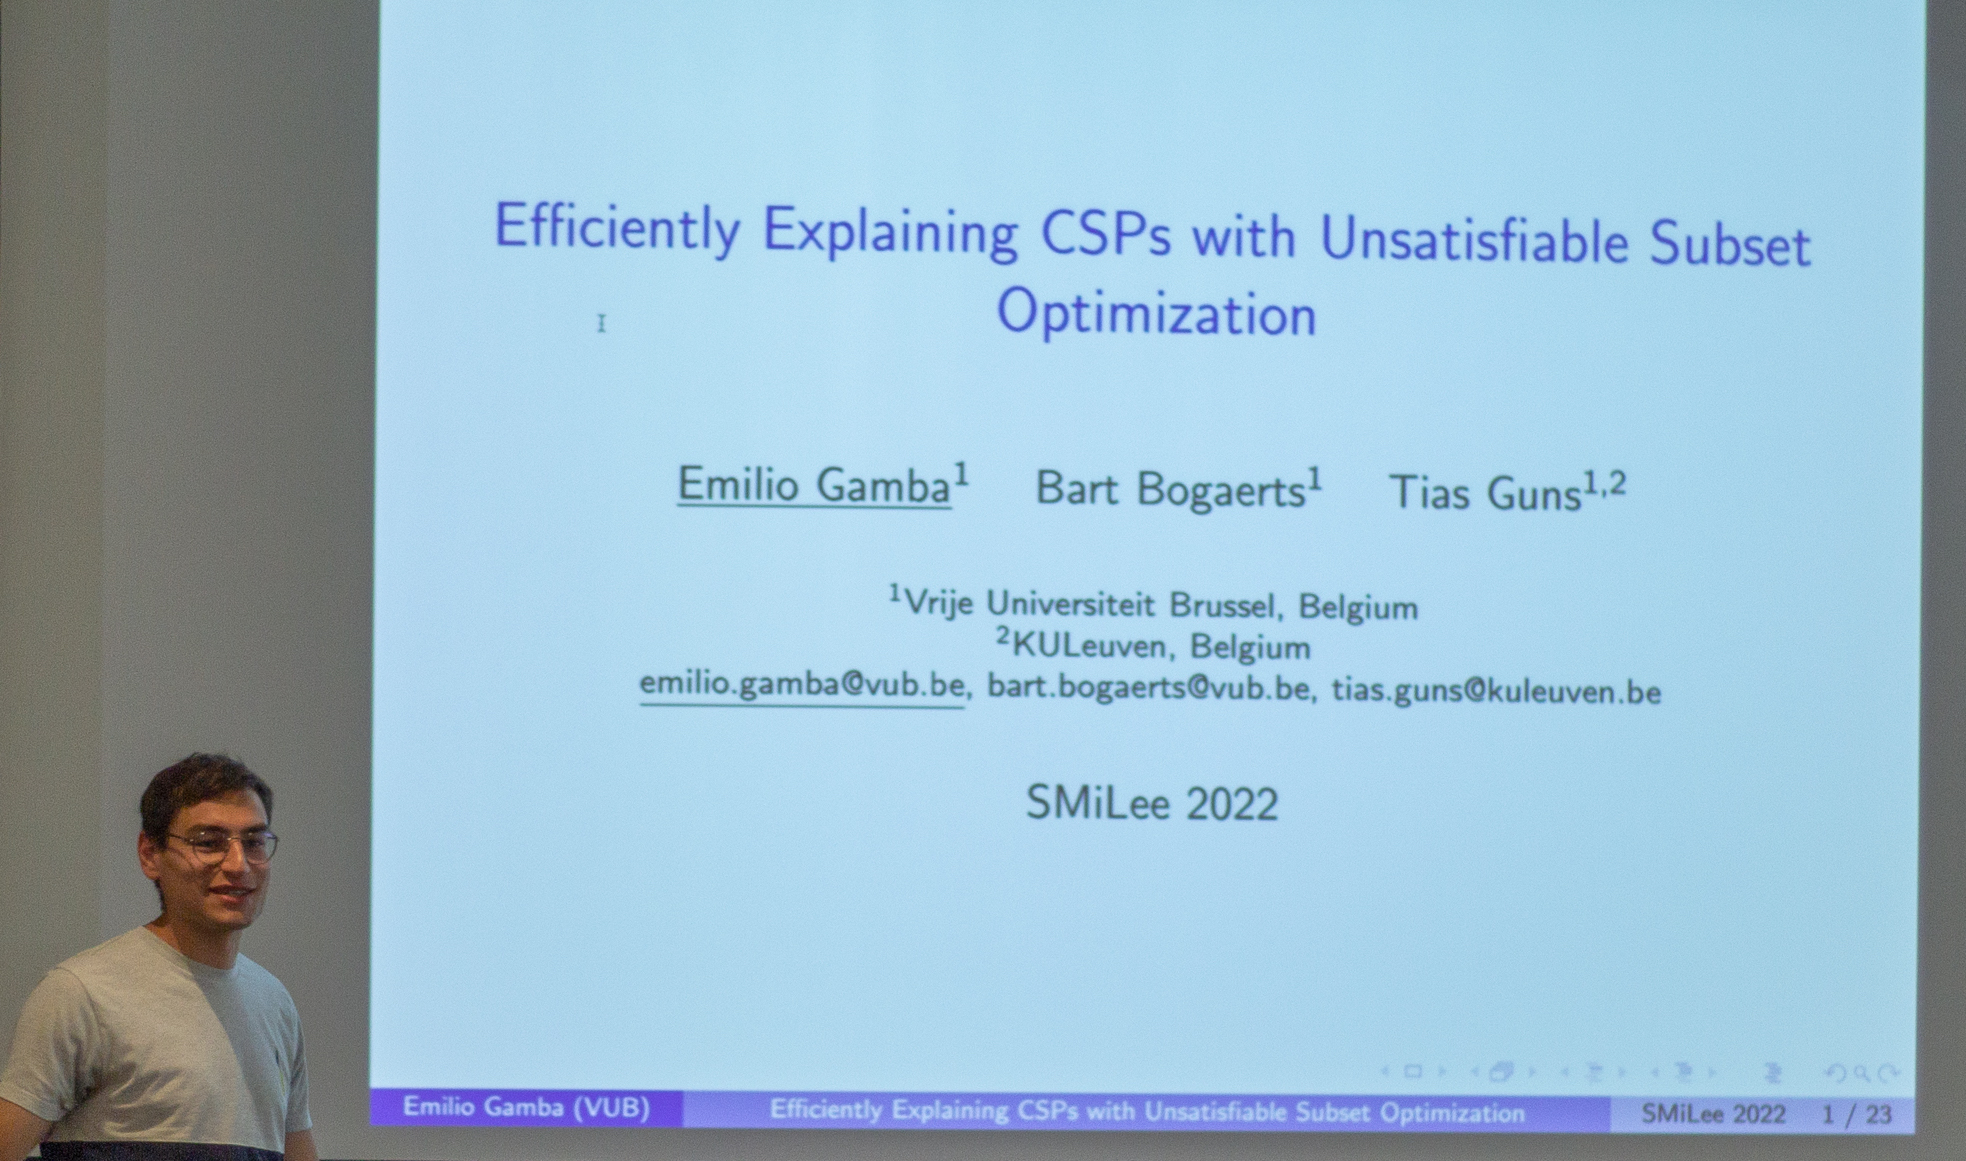
\includegraphics[width=\textwidth]{figures/emilio.jpg}
		}
		 					\only<3>{
			
\includegraphics[width=0.5\textwidth]{figures/emilio_hockey.jpeg}
		}
		 					\only<4>{
			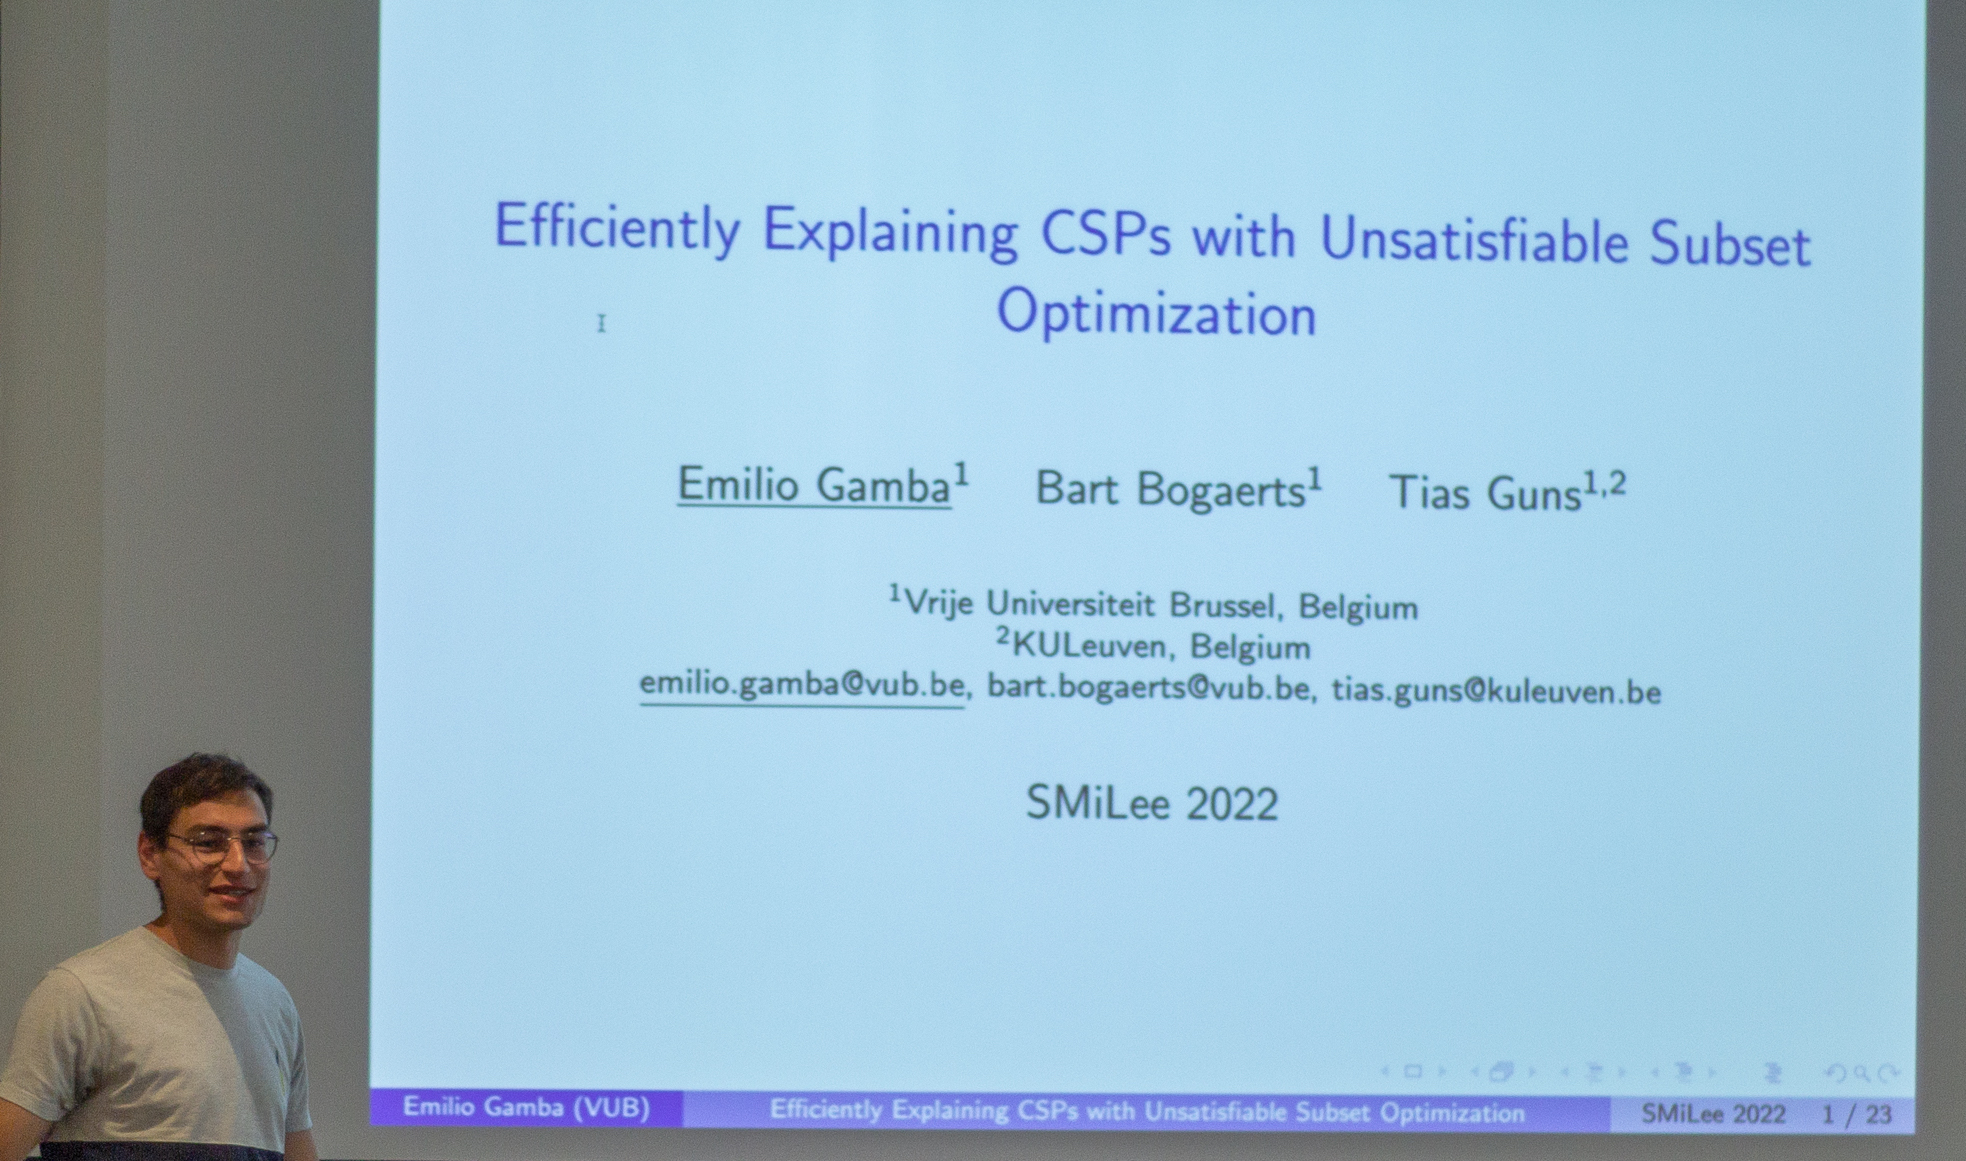
\includegraphics[width=\textwidth]{figures/emilio.jpg}
		}
		\end{figure}
	\end{minipage} 
	\begin{minipage}{.48\textwidth}
	\begin{center}
	\textbf{Emilio Gamba}
	\end{center}\only<2->{
		\begin{itemize}
			\item Joint PhD VUB - KU Leuven
			\item Team Tias 
			\only<3->{\item \textbf{Hobbies:} Field hockey, cycling, cooking and ... eating}
			\only<4->{\item \textbf{Topics:} Constraint Programming, Explainability, Machine Learning}
		\end{itemize}
	}
	\end{minipage}
\end{frame}

\begin{frame}
		\begin{minipage}{.49\textwidth}
{\small\textbf{\emph{Step-wise explanations of CSPs}}}
		\end{minipage}
		\begin{minipage}{.49\textwidth}
	{\small\textbf{\emph{Explanation} (Sudoku Assistant)}}
	\end{minipage} 					\vspace*{10pt}
	
\begin{minipage}{.49\textwidth}
{\footnotesize
\textbf{Motivation}
\begin{itemize}
	\item Explain solutions of CSPs \emph{step-by-step} 
	\item An explanation should be \emph{simple} to \textit{verify} and \emph{understand}.
\end{itemize}
\textbf{Application}
\begin{itemize}
	\item Tutoring system
	\item Explaining schedules, configurations, solution of Constraint Sat / Opt. Problems to users
\end{itemize}}
\end{minipage}\hfill
\begin{minipage}{.49\textwidth}
	\begin{figure}[H]
	
\includegraphics[width=0.9\textwidth]{figures/sudoku_assistant_overview.png}
\end{figure}
	\begin{figure}[H]
	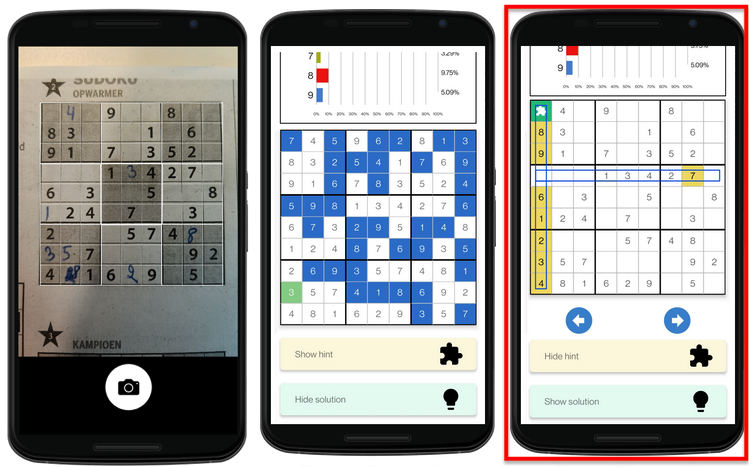
\includegraphics[width=0.9\textwidth]{figures/sudoku_assistant_pipeline.png}
	\caption{{\footnotesize Sudoku Assistant:  An AI-powered app to help solve pen-and-paper Sudokus}}
\end{figure}
\end{minipage} % \vspace{5pt}
\end{frame}

\begin{frame}
	\begin{minipage}{.49\textwidth}
				{\small\textbf{\emph{Explanation Features}}}
	\end{minipage}
	\begin{minipage}{.49\textwidth}
	{\small\textbf{\emph{Explanation Preference Learning}}}
	\end{minipage} 					\vspace*{30pt}
	
\begin{minipage}{.45\textwidth}
	\begin{figure}
	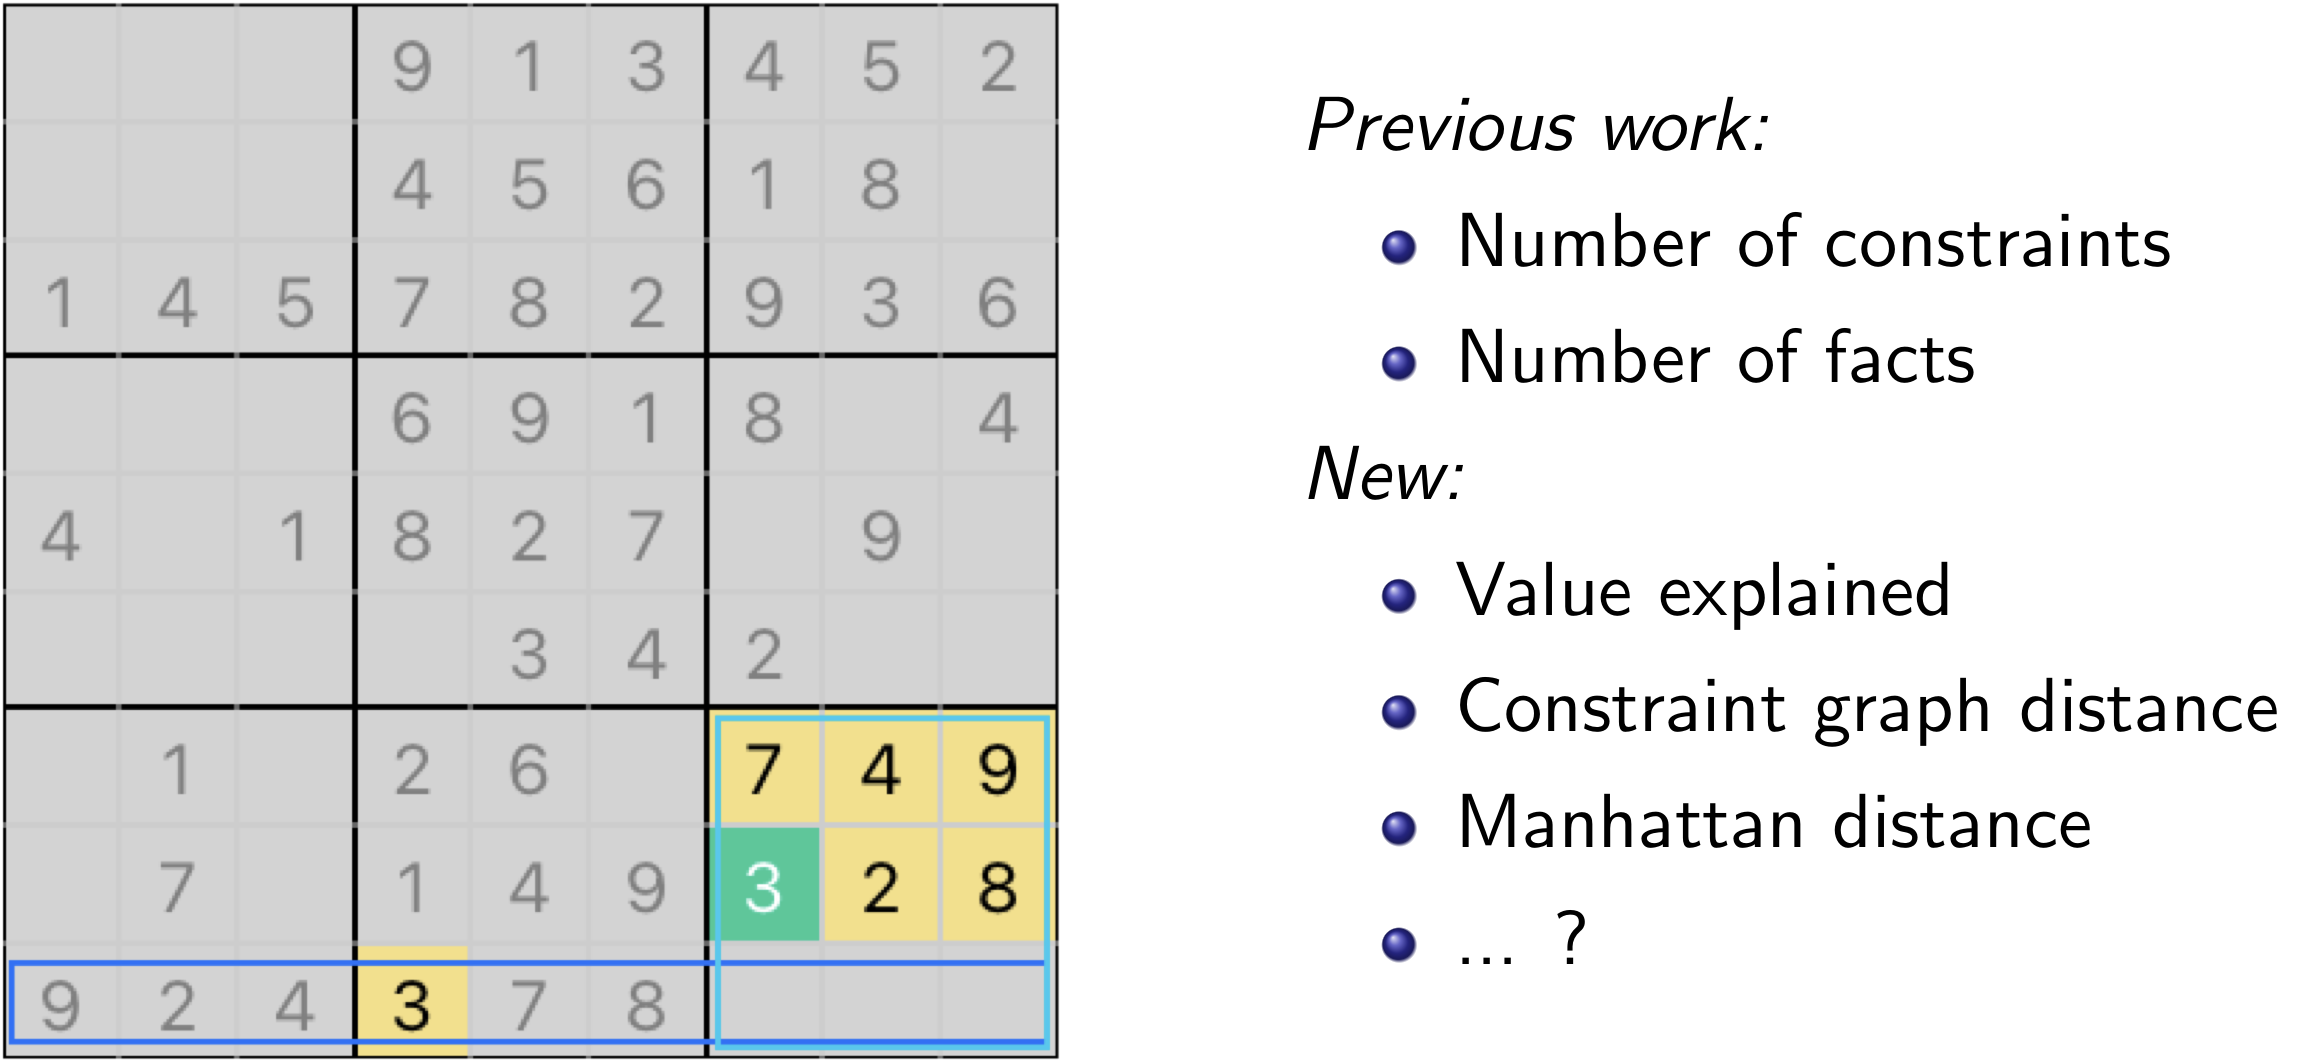
\includegraphics[width=\textwidth]{figures/explanation_features.png}
	\end{figure}
\end{minipage}\hfill
\begin{minipage}{.45\textwidth}
	\begin{figure}[H]
			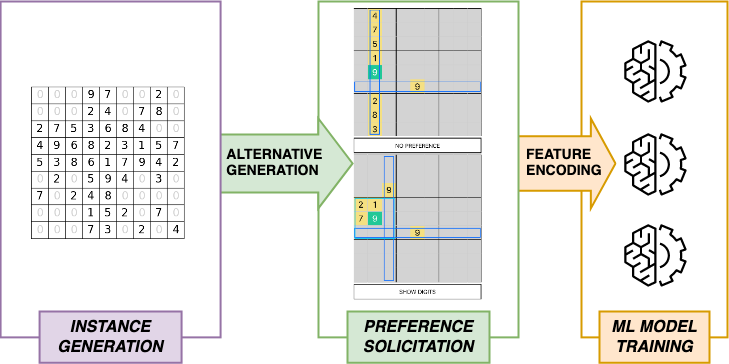
\includegraphics[width=\textwidth]{figures/ml_pipeline.png}
	\end{figure}
\end{minipage}

\begin{center}

\end{center}

\begin{figure}[H]

\end{figure}
\end{frame}

%
%				
%	\begin{frame}
%		\frametitle{Future work}
%		\begin{itemize}
%			\item How to integrate the trained ML model into OCUS generation to \emph{efficiently} compute preferred explanation?
%			\item Learning to rank approaches for ranking explanations and selecting the best one.
%			\item User-preferences: take into account user information, i.e. experience, ...?
%%			\item Inverse optimisation?
%			\item Inverse optimization where given a set of preferred explanations, we want to compute a cost-function.
%		\end{itemize}
%	\end{frame}
%			
%		\begin{frame}[allowframebreaks]
%			\frametitle{References}
%			\bibliographystyle{named}
%			\bibliography{refs,references}
%		\end{frame}		
	
	\end{document}
	